%%%%%%%%%%%%%%%%%%%%%%%%%%%%%%%%%%%%%%%%%
% 8/22 _3suW10W
% 8/28 _3suW11T

\documentclass[letterpaper]{article}
\usepackage[paperwidth=8.5in, paperheight=11in]{geometry}
\linespread{1.2}
\normalsize

\usepackage[utf8]{inputenc}

\usepackage{indentfirst}
\usepackage[utf8]{inputenc}
\usepackage{geometry}

\usepackage{amsmath,amsfonts,amsthm} % Math packages

\usepackage[english]{babel}
\usepackage[autostyle]{csquotes}

%\usepackage{spverbatim}

\usepackage{listings}
\usepackage{lstautogobble}

\lstset{basicstyle=\ttfamily,
	mathescape=true,
	escapeinside=||,
	autogobble,
	xleftmargin=0.7in,
	xrightmargin=.25in}

\usepackage{graphicx}

\usepackage[export]{adjustbox}

\usepackage{amsfonts} % if you want blackboard bold symbols e.g. for real numbers

\usepackage{amsmath}
\usepackage{chngcntr}
\usepackage{wrapfig}
\usepackage{caption}
\usepackage{subcaption}

%\usepackage{subfig}




\numberwithin{equation}{section} % Number equations within sections (i.e. 1.1, 1.2, 2.1, 2.2 instead of 1, 2, 3, 4)
\numberwithin{figure}{section} % Number figures within sections (i.e. 1.1, 1.2, 2.1, 2.2 instead of 1, 2, 3, 4)
\numberwithin{table}{section} % Number tables within sections (i.e. 1.1, 1.2, 2.1, 2.2 instead of 1, 2, 3, 4)

\title{	
	\normalfont \normalsize 
	\huge The Convergence of IDLA to a Circle \\ % The assignment title
}

\author{Jean-Luc Thiffeault and Ruojun Wang} % Your name

\date{\normalsize\today} % Today's date or a custom date

\begin{document}
	
\maketitle % Print the title
	

\section{An IDLA Simulation and the Boundary}

\subsection{An IDLA Simulation with N Particles}

Internal diffusion-limited aggregation (IDLA) is (?) a cluster growth process in which particles start at one or more sources within a cluster, diffuse outward, and are added to the cluster at the first site outside it they reach. (refer?) 

\subsubsection{Particles move in 8 directions}
I started from  MATLAB codes given by Professor Thiffeault. To beign, we prepare a grid quadrant where the particles can perform the IDLA process:

\begin{lstlisting}
    Ngrid = ceil(1.2*sqrt(Npart)); 
	grid0 = Ngrid+1;                
	grid = zeros(2*Ngrid+1);
	x = -Ngrid:Ngrid;
\end{lstlisting}

%\begin{spverbatim}

%\end{spverbatim}

\noindent
where \texttt{Npart} represents the total number of particles that take part into the simulation. \texttt{Ngrid} represents the length of one side of grid quadrant. We let \texttt{grid0} be the center of the grid quadrant and generate an array with size \texttt{2*Ngrid+1}; a \texttt{Ngrid*Ngrid} grid quadrant is then set up. Core codes to simulate IDLA process are as following: 

\begin{lstlisting}
    drift = [0 0];
    for i = 1:Npart
	  X = [0 0];
      while 1
	    X = X + (randi(3,1,2)-2) + drift;	    
	    if ~grid(X(1)+grid0,X(2)+grid0)
	      grid(X(1)+grid0,X(2)+grid0) = 1;
	      break
        ...
\end{lstlisting}

\noindent
In this for loop, we start the first particle from the location \texttt{X = [0 0]}, which would locate at the center \texttt{grid0} of the quadrant we set previously. Then inside the while loop generates the coordinate that the next particle would locate. As the definition of IDLA process states, the next particle would move due to a random direction realized by \texttt{(randi(3,1,2)-2)}. A drift \texttt{drift} might be added to effect the final shape of the particles could form; the direction of drift can be given by \texttt{drift = [0 0]} before the for loop. The codes in if statement just says the particle would keep moving due to \texttt{(randi(3,1,2)-2)} until it finds an unoccupied grid to settle down. An occupied grid would be marked as "1" then. In this first simulation, we want the particles to move in 8 directions randomly (i.e. up, down, left, right, upper left, upper right, lower left, lower right). The results of the simulation are shown in Fig.1.1. We can observe that with the growth of the number of particles which participate in the IDLA process, the boundary of the shape tends to be circular, and hence such a convergence to a circle intrigues us to do further study.

\begin{figure}[htbp]
	\centering
	\begin{subfigure}[b]{0.3\textwidth}
		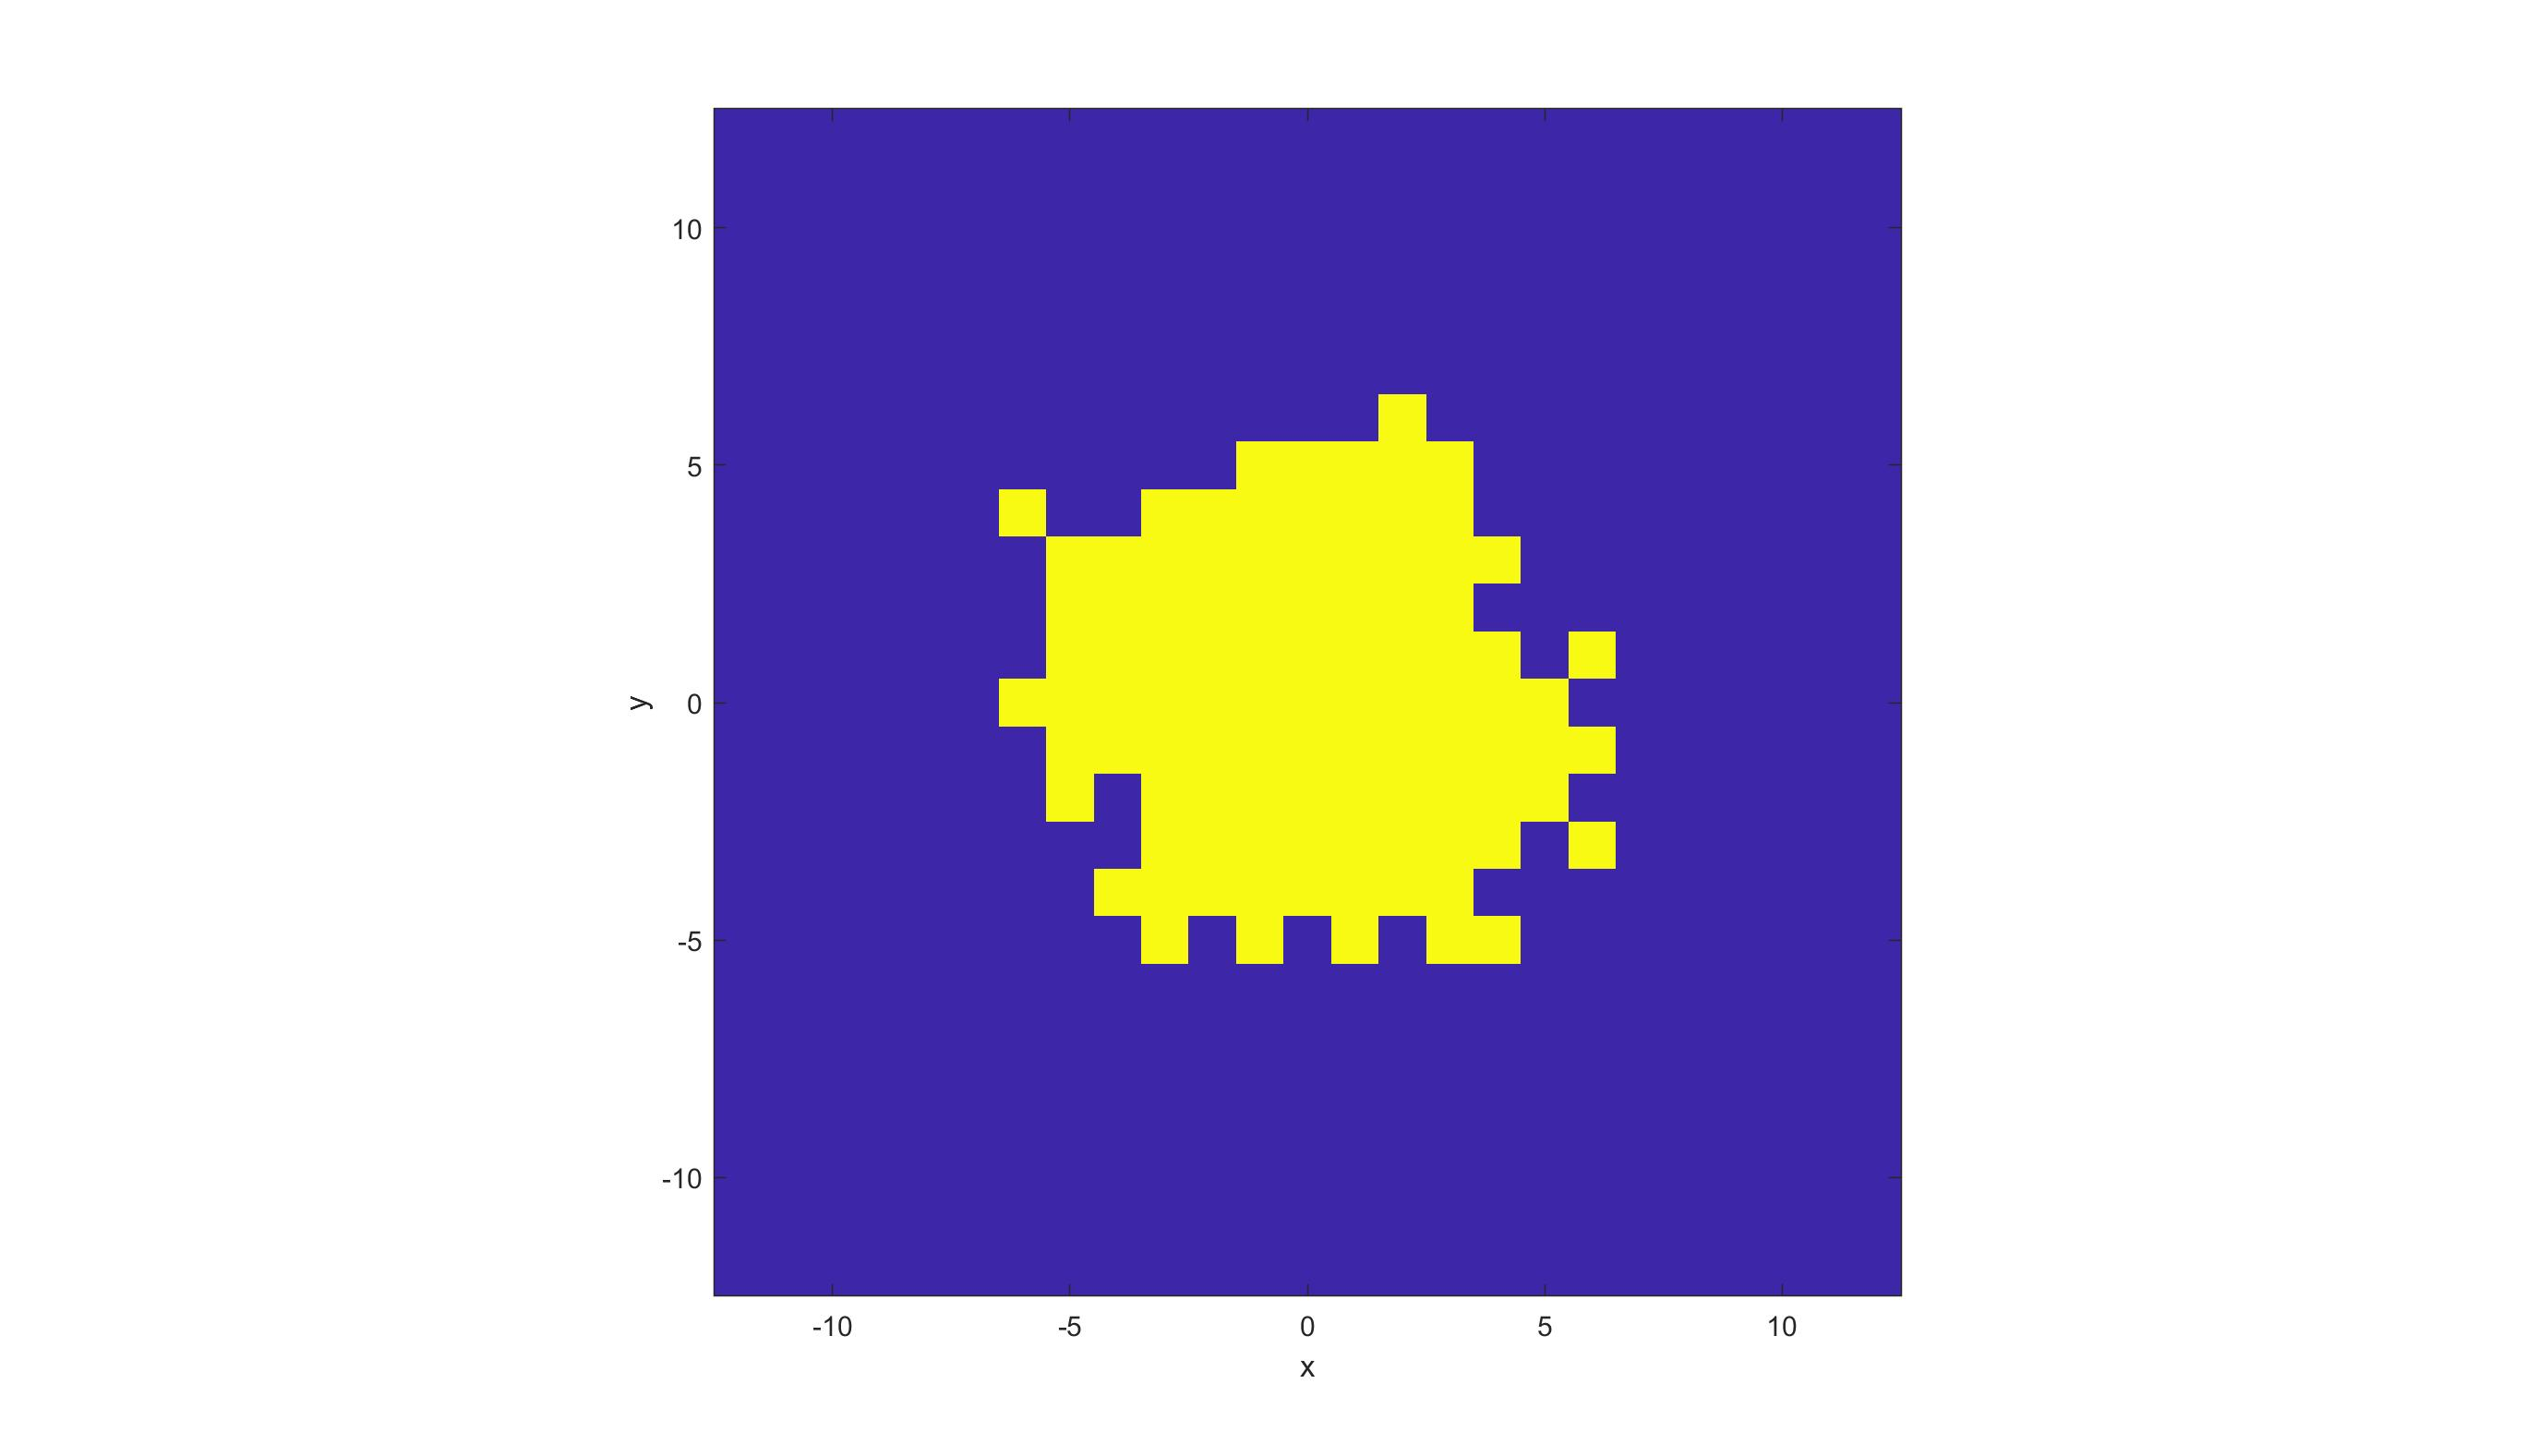
\includegraphics[width=\textwidth]{8direct_Npart100_3suW11T}
		\caption{\texttt{Npart = 100}}
		\label{8direct_Npart100_3suW11T}
	\end{subfigure}
	\begin{subfigure}[b]{0.3\textwidth}
		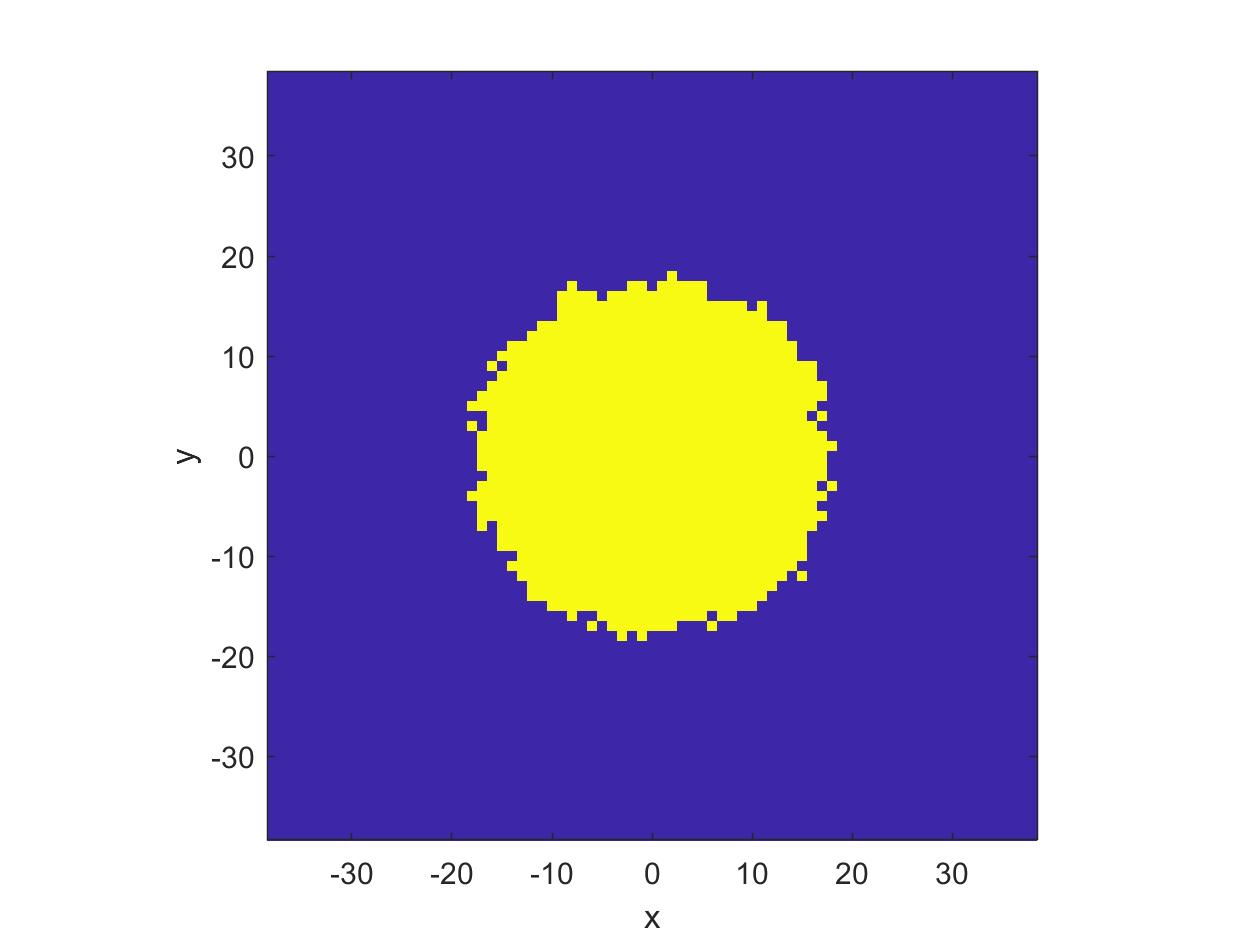
\includegraphics[width=\textwidth]{8direct_Npart1000_3suW11T}
		\caption{\texttt{Npart = 1000}}
		\label{8direct_Npart1000_3suW11T}
	\end{subfigure}
	\begin{subfigure}[b]{0.3\textwidth}
		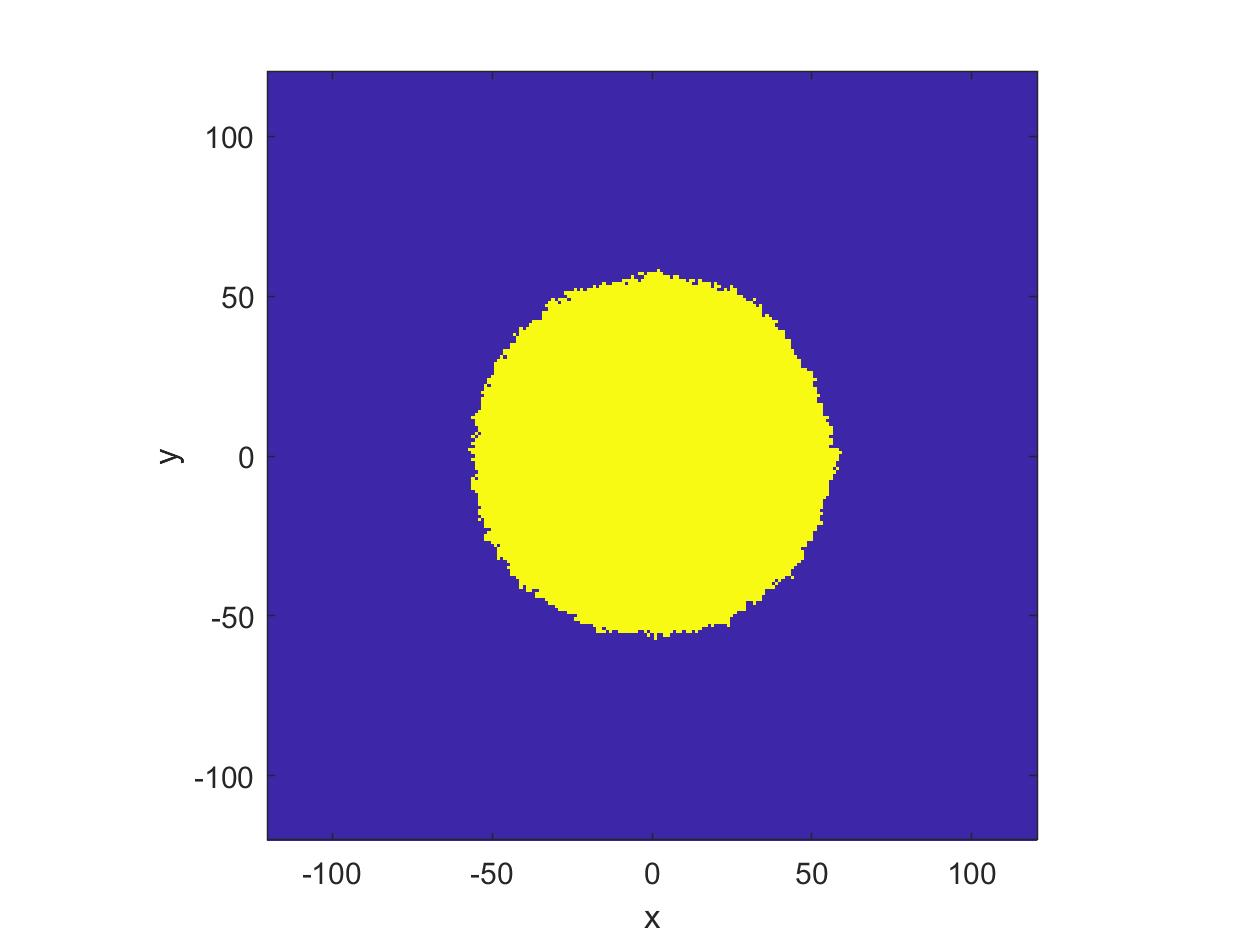
\includegraphics[width=\textwidth]{8direct_Npart10000_3suW11T}
		\caption{\texttt{Npart = 10000}}
		\label{8direct_Npart10000_3suW11T}
	\end{subfigure}
	\caption{IDLA simulation with 8 directions}
	\label{IDLA simulation with 8 directions}
\end{figure}
	



\subsection{Particles move in 4 directions}
My first task is to restrict the motion of direction for each particles which involve in IDLA process. We would like to see if the boundary of the occupied region is still converging to a circle by restricting the particles to choose a random motion in 4 directions. That is, we eliminate the diagonal motion of particles (i.e. upper left, upper right, lower left, lower right). The MATLAB codes to realize this are:

\begin{lstlisting}
    v_dir = [1 0; 0 1; -1 0; 0 -1];
    n_dir = 4;
    
    for i = 1:Npart
      X = [0 0];
      while 1
    
      d = randi(n_dir);
    
      X(1) = X(1) + v_dir(d, 1) + drift(1); 
      X(2) = X(2) + v_dir(d, 2) + drift(2);
      ...
      
\end{lstlisting}

\noindent
Here, we prepare a 4*2 matrix containing 4 vectors which represent four directions that a particle can move along. Then similarly as the case shown in the motion with 8 directions, inside the for loop, we start from the center of the grid quadrant \texttt{[0 0]}. After determining a random number inside a list consisting 1 to 4, we are able to select a vector in the 4*2 matrix and then determine the direction of the particle moves along. The results of the simulation are shown in Fig.1.2.

%\begin{figure}[h]
%	\begin{subfigure}{0.5\textwidth}
%		\centering
%		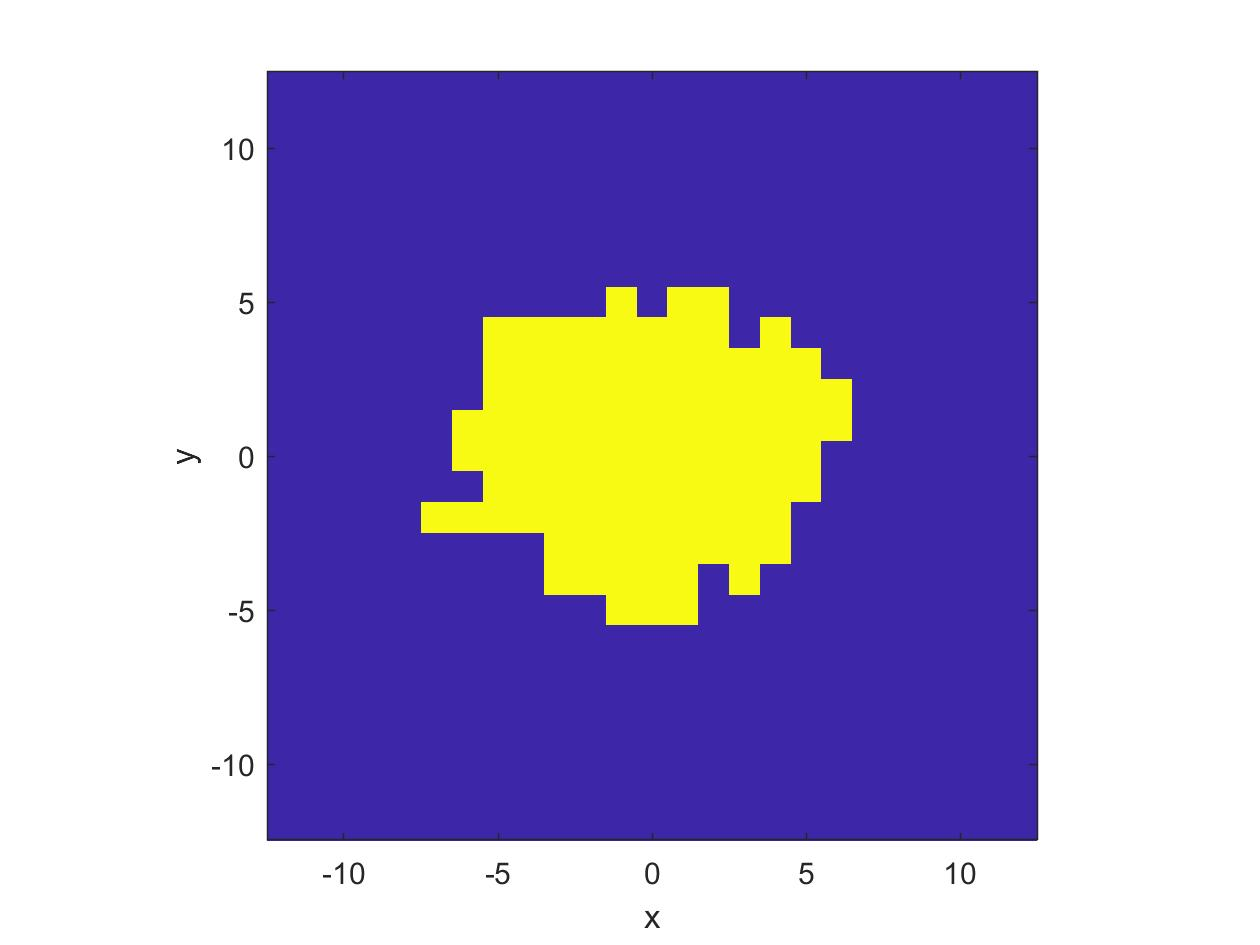
\includegraphics[width=0.7\linewidth]{4direct_Npart100_3suW11T}
%		\caption{\texttt{Npart = 100}}
%		\label{fig:4directnpart1003suw11t}
%	\end{subfigure}
%	
%	\begin{subfigure}{0.5\textwidth}
%		\centering
%		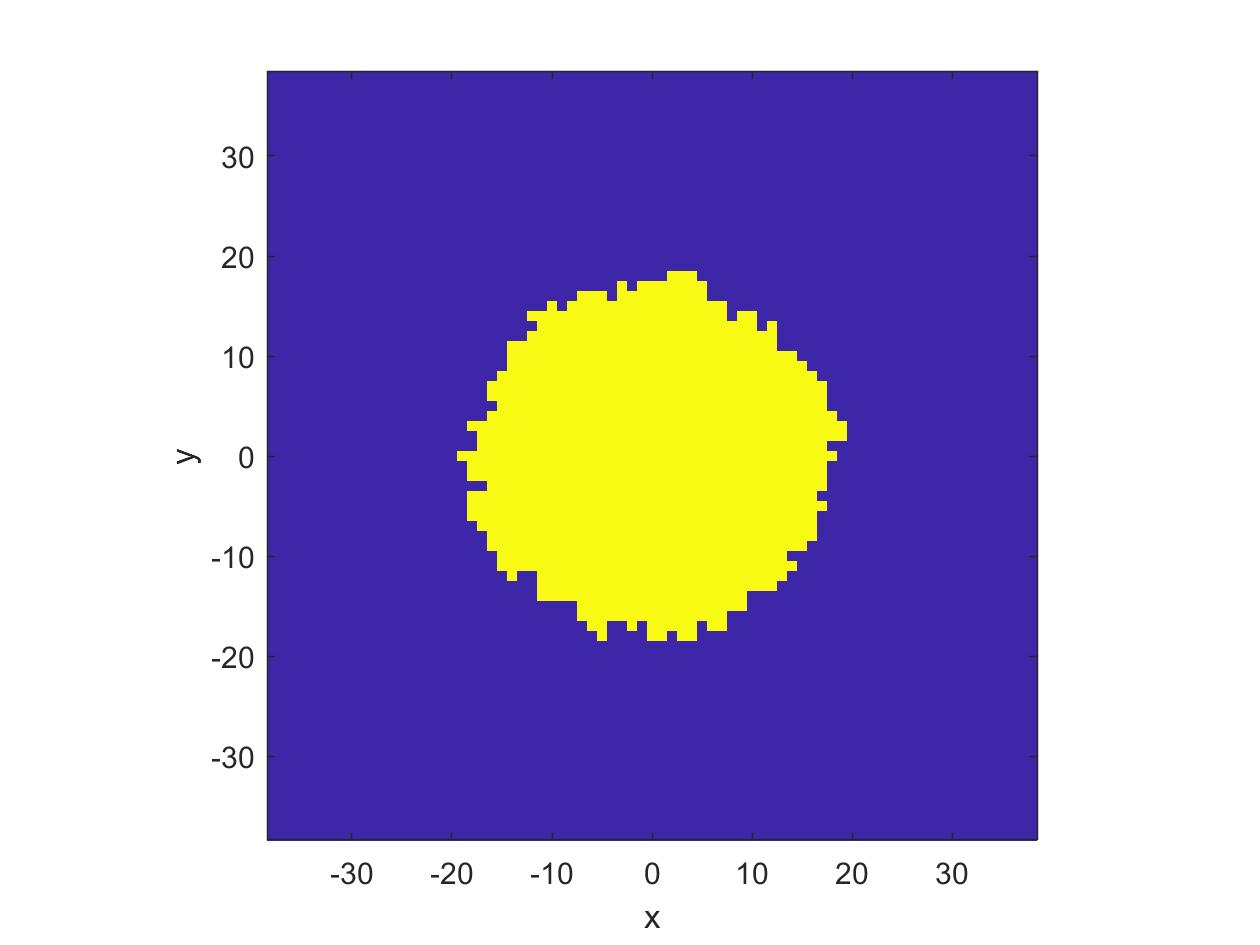
\includegraphics[width=0.7\linewidth]{4direct_Npart1000_3suW11T}
%		\caption{\texttt{Npart = 1000}}
%		\label{fig:4directnpart10003suw11t}
%	\end{subfigure}
%	
%	\begin{subfigure}{0.5\textwidth}
%		\centering
%		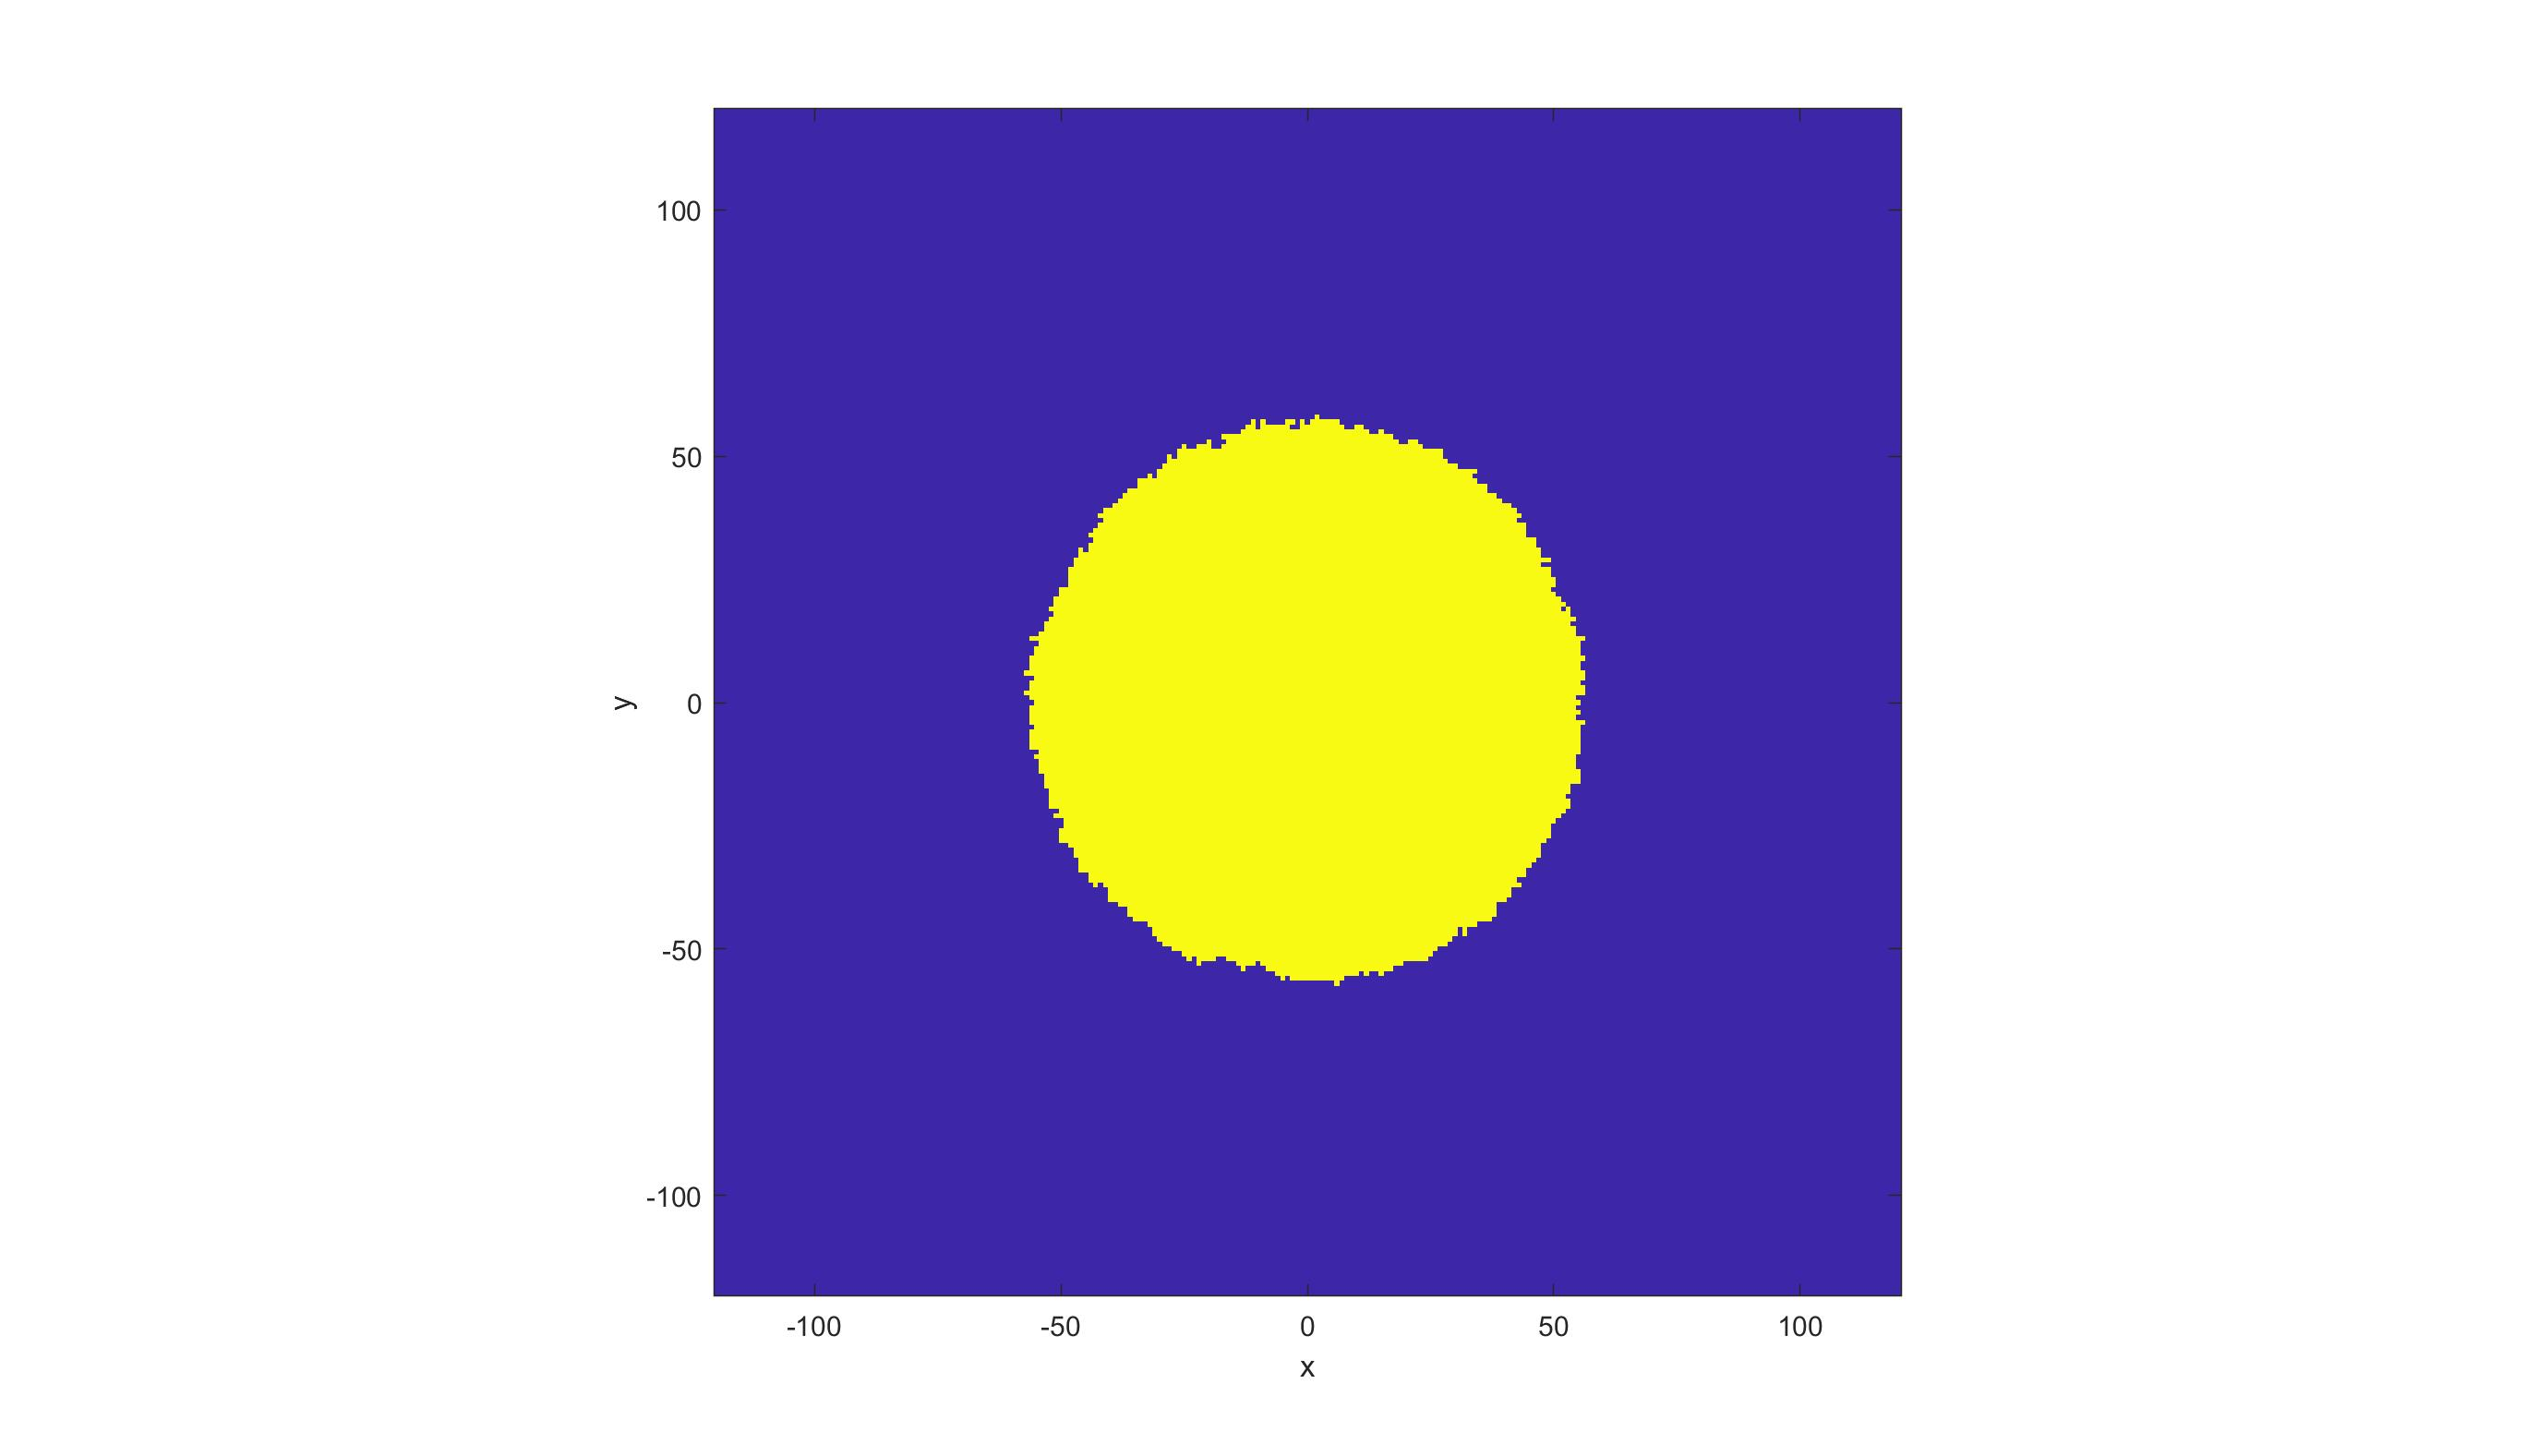
\includegraphics[width=0.7\linewidth]{4direct_Npart10000_3suW11T}
%		\caption{\texttt{Npart = 10000}}
%		\label{fig:4directnpart100003suw11t}
%	\end{subfigure}
%	
%	\caption{IDLA simulation with 4 directions}
%	\label{fig:image2}
%\end{figure}

\begin{figure}[htbp]
	\centering
	\begin{subfigure}[b]{0.3\textwidth}
		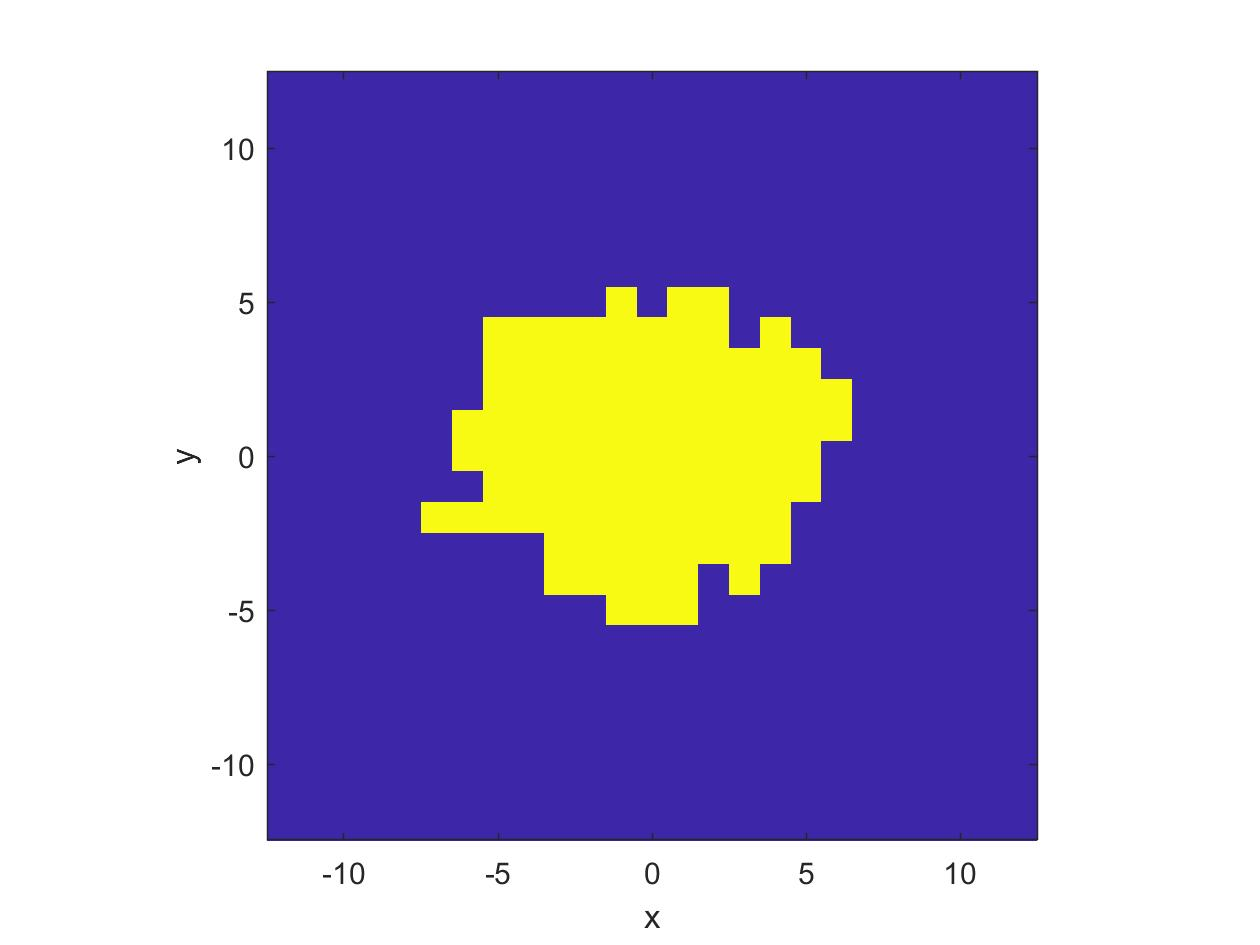
\includegraphics[width=\textwidth]{4direct_Npart100_3suW11T}
		\caption{\texttt{Npart = 100}}
		\label{4direct_Npart100_3suW11T}
	\end{subfigure}
	\begin{subfigure}[b]{0.3\textwidth}
		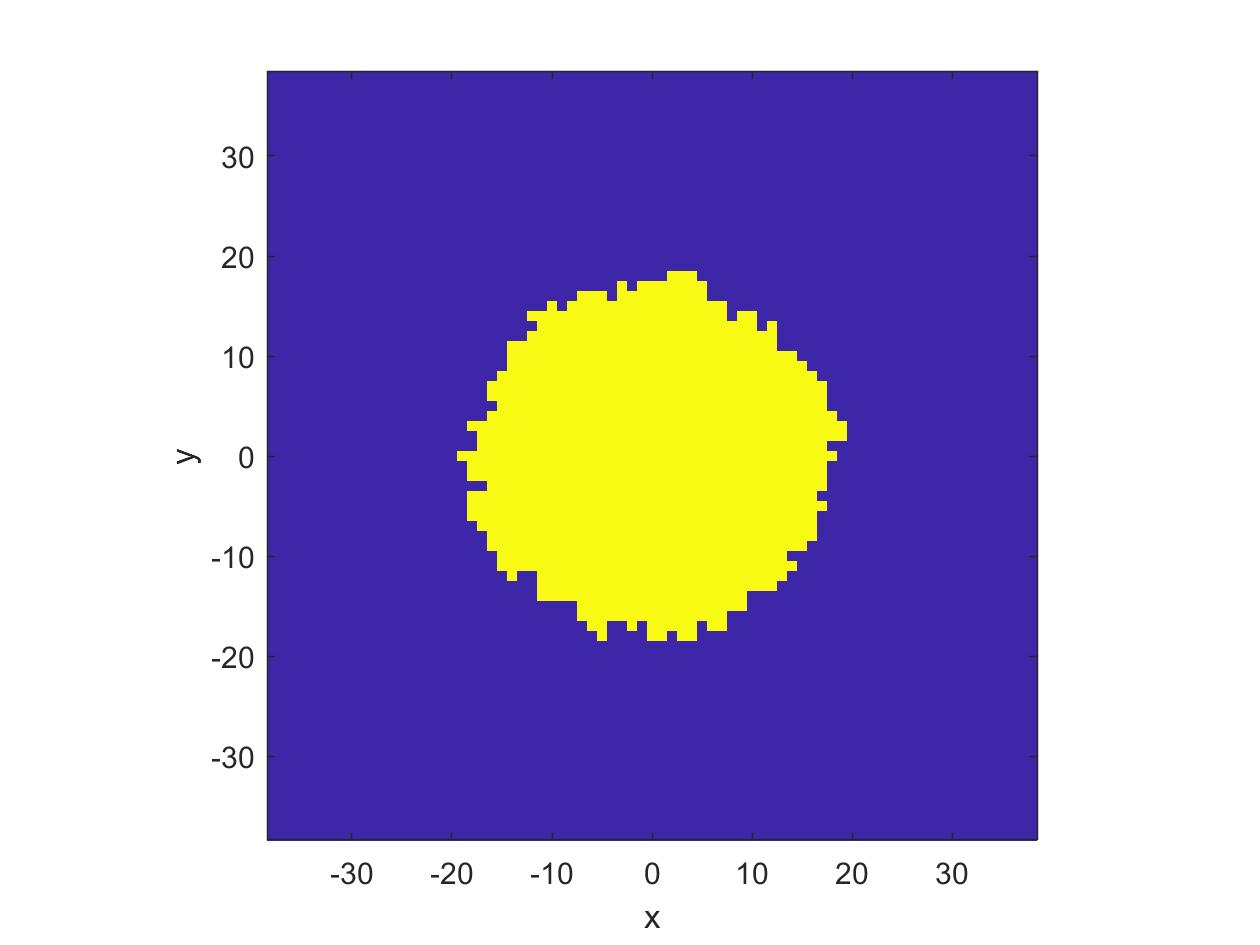
\includegraphics[width=\textwidth]{4direct_Npart1000_3suW11T}
		\caption{\texttt{Npart = 1000}}
		\label{4direct_Npart1000_3suW11T}
	\end{subfigure}
	\begin{subfigure}[b]{0.3\textwidth}
		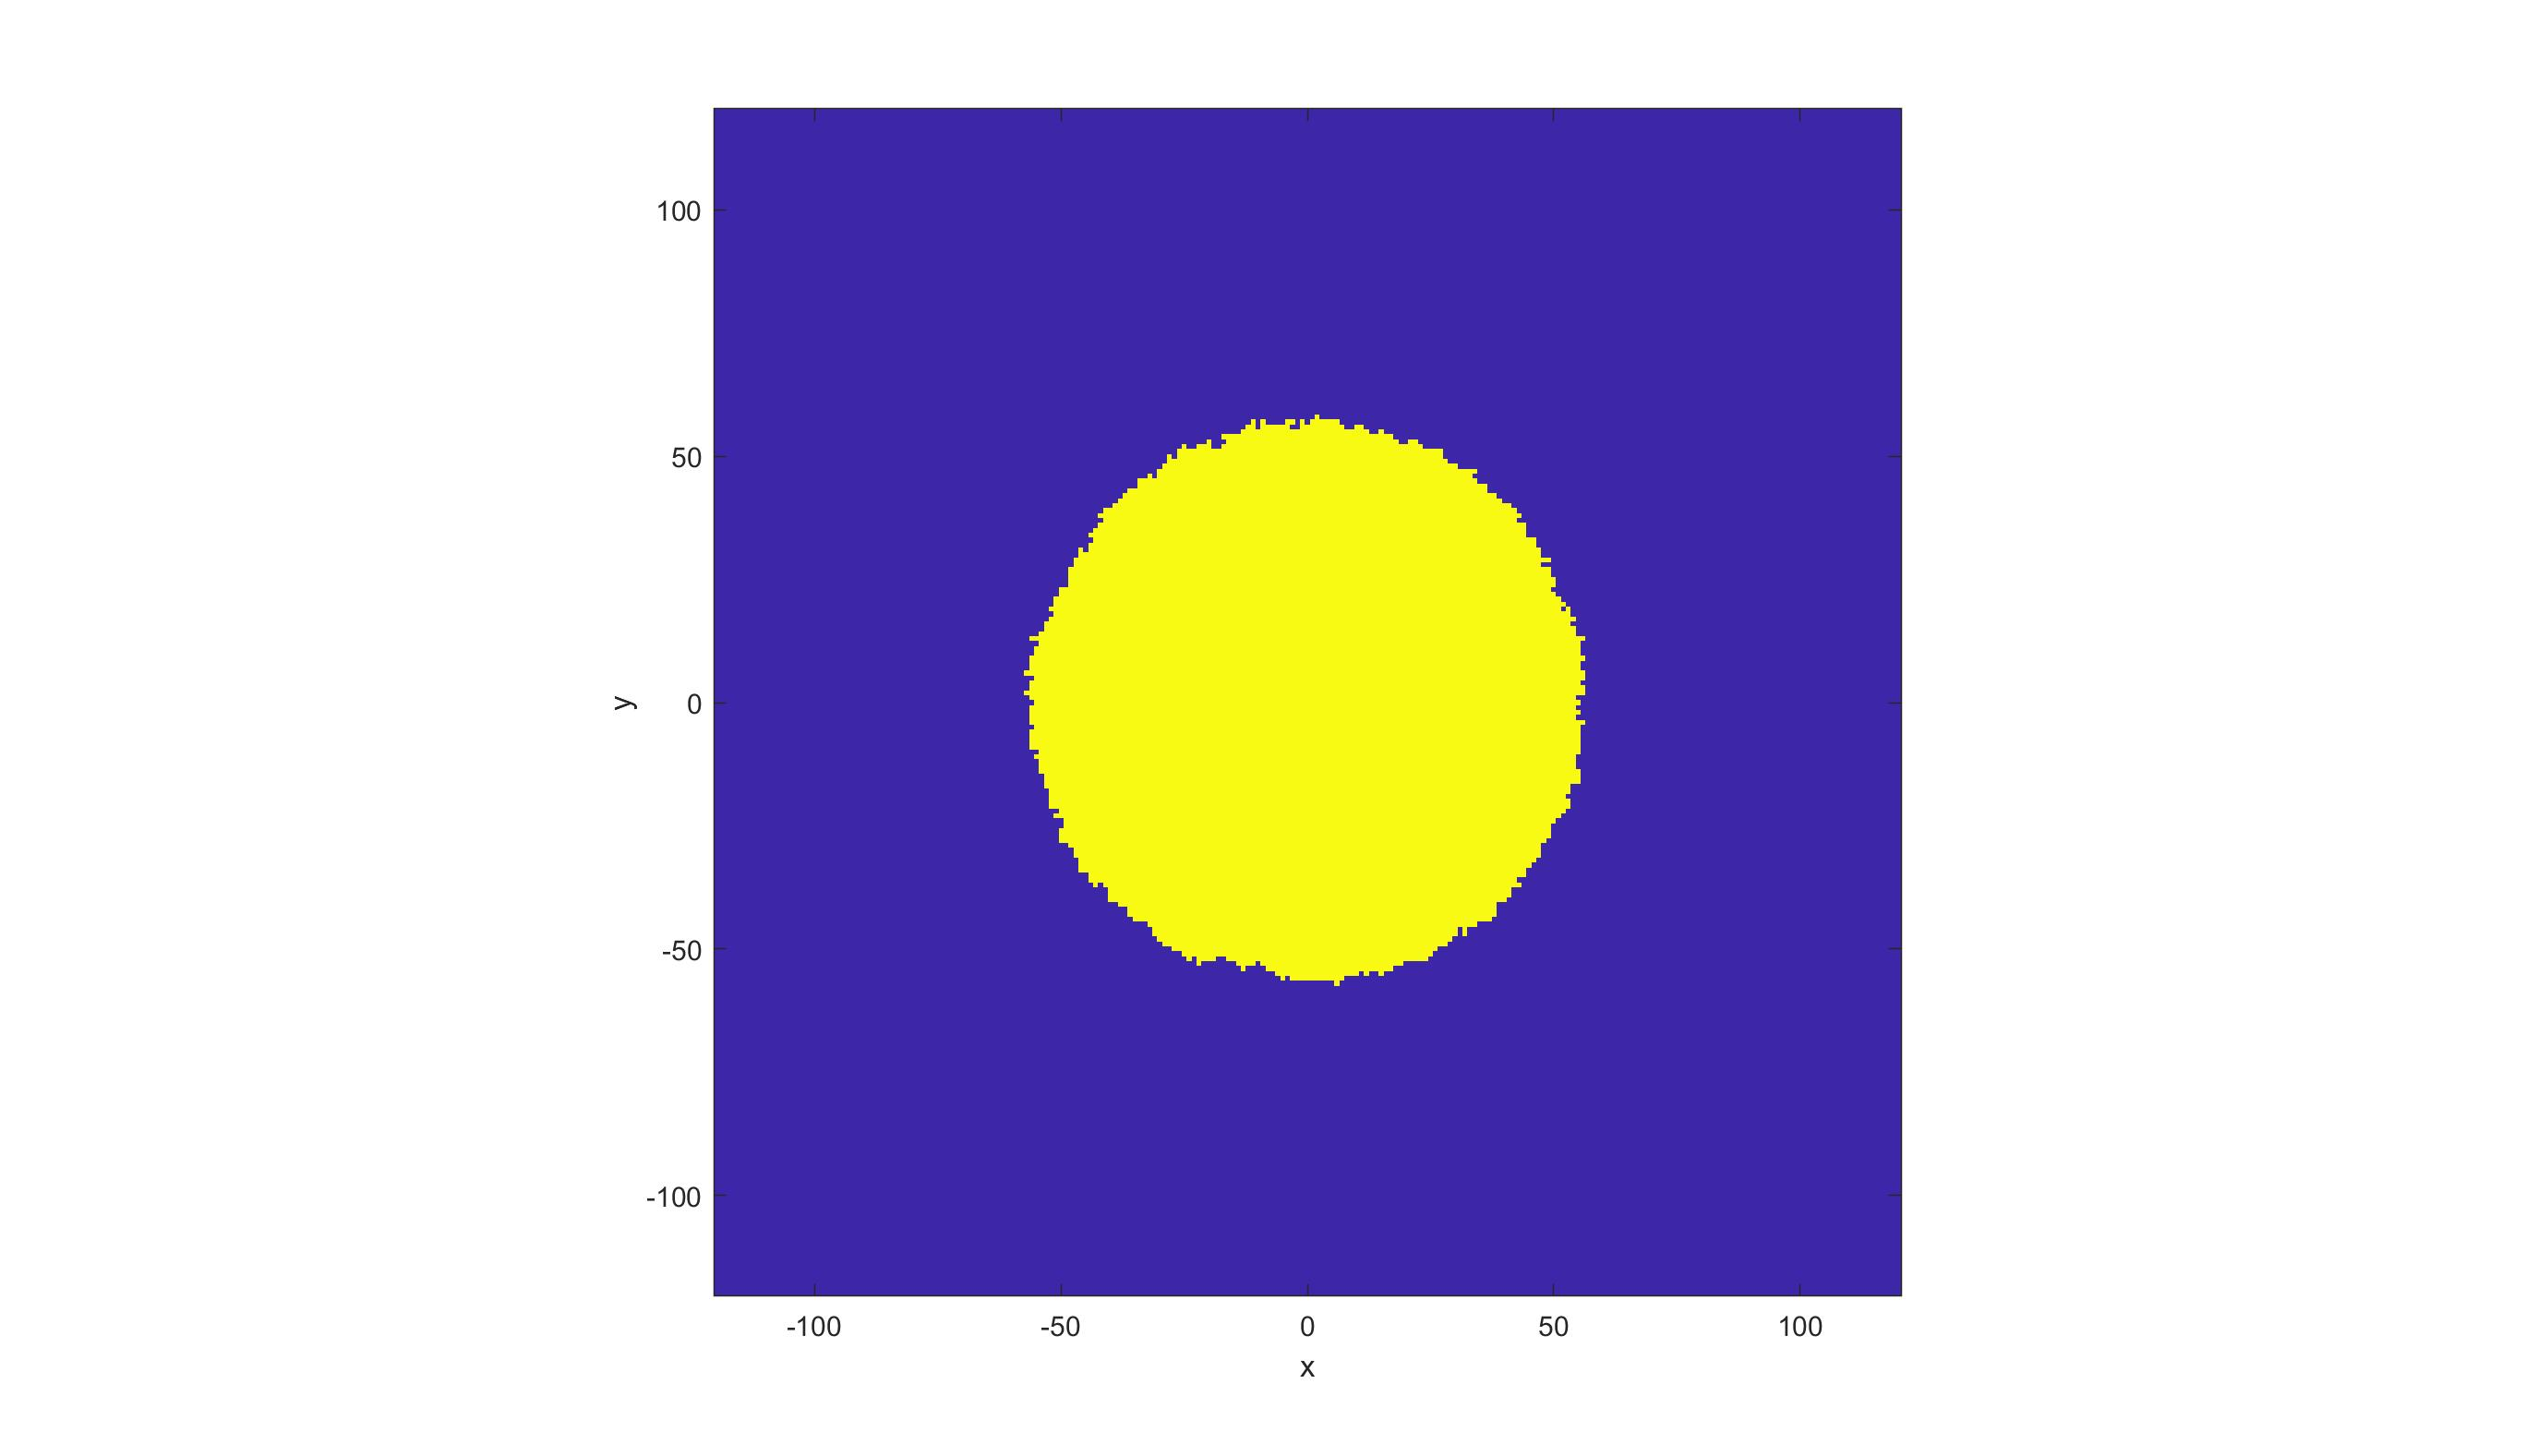
\includegraphics[width=\textwidth]{4direct_Npart10000_3suW11T}
		\caption{\texttt{Npart = 10000}}
		\label{4direct_Npart10000_3suW11T}
	\end{subfigure}
	\caption{IDLA simulation with 4 directions}
	\label{IDLA simulation with 4 directions}
\end{figure}

\noindent
We could then observe that a IDLA simulation also produce a final occupied region which converges to a circle, as the number of particles which participated grows (Fig.1.2).

\subsection{Boundary of the Occupied Region}
From the graph generated by MATLAB codes, we observe that the boundary of the shape constructed by the IDLA process tends to be smooth and to imitate a circle, as the value of \texttt{Npart} (the number of particles) become larger. We want to understand to what extent the shape constructed by the process converges to a circle. We start by selecting out the pixels which constitute the boundary of the occupied region and mainly focus on these pixels. Three different algorithms are tried to remain the boundary only as the IDLA process evolves.

\subsubsection{Three Algorithms to Build the Boundary}

\paragraph{Build entire boundary.}
The idea here is to start from an occupied grid on the boundary (for example, one on the boundary which has the same horizontal coordinate as the center grid), to examine its neighbor occupied grids, to choose the next one which is on the boundary, to examine the neighbors based on this next grid, and hence to find all the grids on the boundary of the occupied region.

(use image maybe?)

\begin{lstlisting}
for k=1:size(bdP,1)  
  if ~(bdP(k,1) == 0 && bdP(k,2) == 0)  
  finish = 0;
  neighb = [bdP(k,1)+1 bdP(k,2); bdP(k,1)-1 bdP(k,2); 
    bdP(k,1) bdP(k,2)+1; bdP(k,1) bdP(k,2)-1; 
    bdP(k,1)+1 bdP(k,2)+1; bdP(k,1)+1 bdP(k,2)-1; 
    bdP(k,1)-1 bdP(k,2)+1; bdP(k,1)-1 bdP(k,2)-1];

    for j=1:8
      if (grid(neighb(j,1), neighb(j,2))==1 && 
      gridB(neighb(j,1), neighb(j,2))==0)  

        if ~((grid(neighb(j,1)+1, neighb(j,2))==1) && 
        (grid(neighb(j,1)-1, neighb(j,2))==1) && 
        (grid(neighb(j,1), neighb(j,2)+1)==1) && 
        (grid(neighb(j,1), neighb(j,2)-1)==1)) 

          bdP = [bdP; neighb(j,1) neighb(j,2)];    
          gridB(neighb(j,1), neighb(j,2))=1;  
          ...
\end{lstlisting}

\noindent
In the first for loop, we prepare the coordinates of all eight neighbors for one particular occupied grid: Since the boundary of the occupied region can be constructed by grids which are only connected diagonally, so to examine the total eight closest grids for one is necessary. If an occupied grid is marked as "1" and an unoccupied one is marked as "0," we can determine the next occupied grid on the boundary by seeing if all its horizontally and vertically connected neighbors are marked as "1."

\paragraph{Build boundary incrementally.} 
This algorithm is designed to examine all the grids on the grid quadrant and select out the grids which construct the boundary only as the occupied region grows. The idea is to come up with a method to tell the difference between the grids inside the region and outside it: the grids which are not on the boundary are surrounded by grids along its four sides, while the grids which are on the boundary have at least one side which does not touch another grid. Hence, as one more particle is added to the process, we could eliminate those which are not considered on the boundary. For example, in Fig.1.3, when the fifth particle is added to the process, we can determine the grid at the center is no longer a grid on the boundary and it should be removed. The MATLAB codes are shown as following: 

\begin{figure}[h]
		\centering
		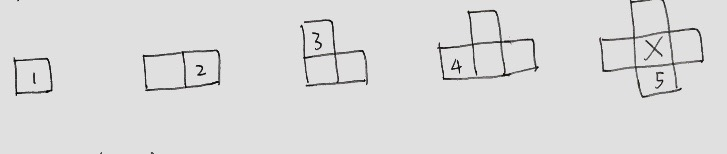
\includegraphics[width=0.7\linewidth]{bdryAlg2}
		\caption{remove a grid which is not considered on the boundary any longer}
		\label{fig:bdryAlg2}
\end{figure}




\begin{lstlisting}
for k = 2:(2*grid0-1)
  for l = 2:(2*grid0-1)
    if grid(k, l) == 1 && grid(k, l+1) == 1 && 
    grid (k, l-1) == 1 && grid (k+1, l) == 1 && 
    grid (k-1, l) == 1
    
      gridB(k, l) = 0; 
      ...
\end{lstlisting}

\noindent
where the grids which are occupied are marked as "1," and those which are not occupied are denoted as "0." By examining if all four neighbors of one grid are marked as "1," we are able to determine whether one grid is considered on the boundary.


\paragraph{Build boundary by Discrete Laplace.}
The third algorithm using Discrete Laplace has the similar idea to the second one. A Discrete Laplace can be written as:

\begin{align} 
(\Delta f)_{i,j} = 4f_{i,j}-f_{i+1,j}- f_{i-1,j}-f_{i,j+1}-f_{i,j-1}
\end{align}

\noindent
Similarly to the second algorithm, the grids which are occupied are marked as "1," and those which are not occupied are denoted as "0." Hence, if $(\Delta f)_{i,j}>0$, the grid with coordinate $(i,j)$ is considered on the boundary. The MATLAB codes can be written as:

\begin{lstlisting}
for k = 2:(2*Ngrid)
  for l = 2:(2*Ngrid)
    delta_f = 4*grid(k, l) - grid(k, l+1) - grid(k, l-1) 
    - grid(k+1, l) - grid(k-1, l);

    if delta_f == 0  
      gridB(k, l) = 0; 
      ...
\end{lstlisting}

In order to see if those three algorithms return the same results regarding the grids on the boundary which are selected out, I also further compare the discretized boundary generated by three algorithms and it turns out they agree with each other.

\subsubsection{The Numerical Standard Deviation}
The standard deviation from the simulation, which is marked by $\sigma_{sim}$, consists of two errors, the geometric error $\sigma_{geom}$ and the statistical error $\sigma_{stat}$. 

\begin{figure}[h]
	\centering
	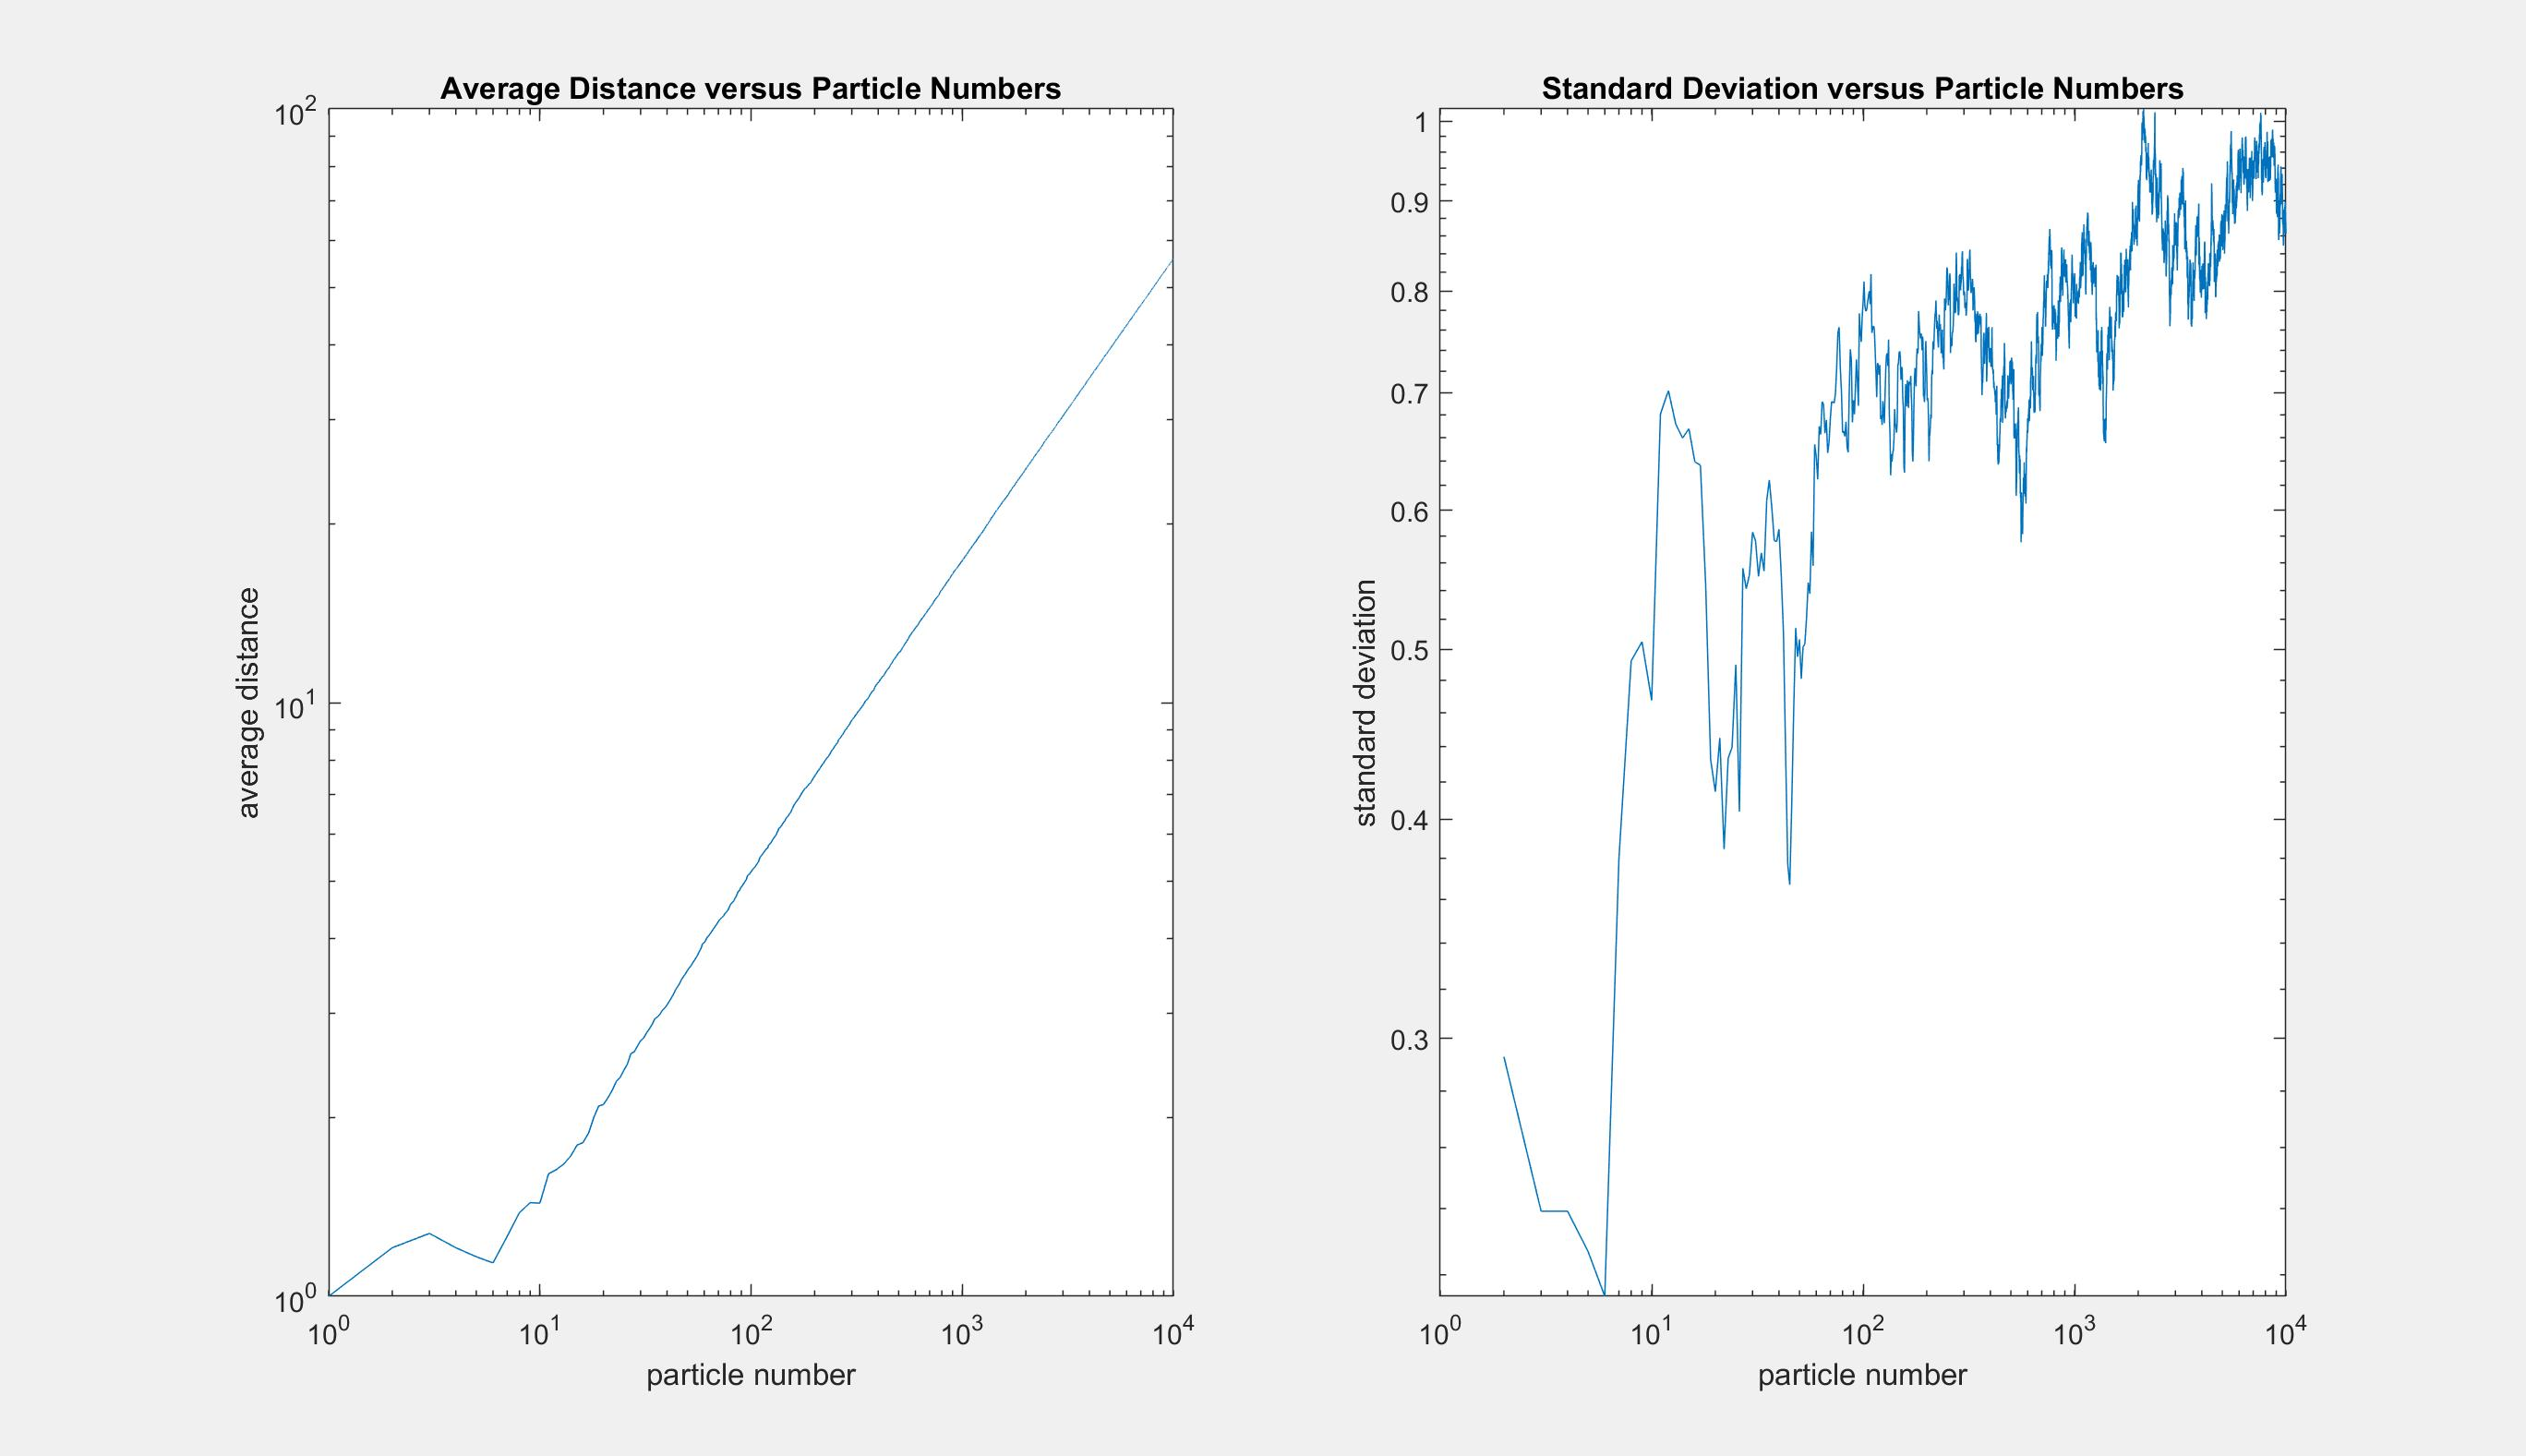
\includegraphics[width=0.7\linewidth]{bdryRandSTD}
	\caption{Average Radius versus Particle Numbers and Standard Deviation versus Particle Numbers when \texttt{Npart=10000}}
	\label{fig:bdryRandSTD}
\end{figure}

\section{The Geometric Error}

A discretized circle can be constructed by two different kinds of algorithms, in order to obtain the geometric error $\sigma_{geom}$. 

\subsection{The Numerical Standard Deviation}

\subsubsection{The \enquote{Nonremove} Case}
We consider a grid (a lattice of circle) in the plane with centers at coordinates $p=(m, n)\in\mathbb{Z}^2$. The center of circle drawn locates at the origin $(0,0)$. Take a circle of radius $R$, centered on the origin. A continuous discretization of the circle is an ordered set of distinct pixels which the boundary of the circle passes through

\begin{align} 
\mathcal{D}_R=(p_{i})_{0 \leq i \leq N-1} = (m_i, n_i)_{0 \leq i \leq N-1},
\end{align}

\noindent
where $m_i$ denotes the horizontal coordinate of the center of a pixel and $n_i$ denotes the vertical one of that.

The algorithm can be realized by MATLAB codes as following: ... Given $R=10000$, $\sigma_{geom}=0.3729$.

	
\subsubsection{The \enquote{Remove} Case}

Another ways to construct a discretized consisting of less pixels occupied than those in the first algorithm. The algorithm can be realized by MATLAB codes: ... When $R=10000$, $\sigma_{geom}=0.2624$, which is smaller than the value obtained from the first algorithm.

\subsection{The Upper Bound of $L_{2}$ Error of the Discretization}

(A derivation of $L_{2}$ Error of the discretization.)

\begin{align} 
\text{Err}_2 \ \mathcal{D}_R=(\frac{1}{N} \sum_{i=0}^{N-1} (m_i^2+n_i^2)-R^2)^{\frac{1}{2}}.
\end{align}


In both algorithm to construct a discretized circle, $\sigma_{geom}$ can be approximated by Err$_2 \ \mathcal{D}_R$ when $R \rightarrow \infty$, since ... Err$_2 \ \mathcal{D}_R$ can be considered as the distance between the center of each pixel $p_i$ and the boundary of the circle which passes through this pixel. We denote Err$_2 \ \mathcal{D}_R$ as $d$ in this case. By computation(...), if the small piece is randomly distributed, the expectation value $\mathbb{E}\ d^2 \approx 0.1667$. 

For both algorithms, a analytical upper bound can be found for $d^2$, which approximately equal to $\sigma_{geom}^2$ when $R \rightarrow \infty$. $\sigma_{geom}^2 \leq \frac{1}{2} \approx 0.5$ and then $\sigma_{geom} \leq 0.7071$.

(We sort pixels into 4 different types as following to lower the upper bound of $d$ ...)

\subsubsection{Sort Pixels into 4 Different Types}
According to the ways that the boundary of the circle passes through each pixel, we can sort $N$ pixels into 4 different types for the upper right quarter of the circle (other three quarters would just be the mirror images of the upper right one with respect to different axises of symmetry). As the algorithm provided above, the center of each pixel is represented by $(m_i, n_i)$. (graph?) The boundary of the circle passing by would have 2 different intersections with a pixel $p_i$. Hence, the four different type of grids can be given by the inequalities restricting the coordinates $(x,y)$ of the intersections. The first kind of pixel is provided by  

\begin{align} 
\text{one intersection: } x=m_i-\frac{1}{2}; \ n_i-\frac{1}{2}\leq y \leq n_i-\frac{1}{2}, \ \text{where} \ y=\sqrt{R^2-(m_i-\frac{1}{2})^2};
\end{align}

... (other inequalities)

(A deviation to find upper bound by evaluating these four types of pixels.) 

\begin{align} 
\sigma_{geom}^2 \leq \frac{1}{2} \approx 0.5
\end{align}

Also, $\sigma_{geom} \leq 0.7071$. (The upper bound is still the same. We need a further improvement.)

\subsubsection{An Observation of the Relation between the Fraction of Each Type of Pixels and Multiples of $R$}

(By derivation, $(1-\frac{1}{\sqrt{2}})R \approx 0.29289 R$ and $\frac{1}{\sqrt{2}}R \approx 0.70711 R$)

\paragraph{The \enquote{Nonremove} Case.}
Given by MATLAB codes, the numerical fraction of the four different type of pixels are 

\begin{align} 
\text{fraction of type 1}=0.29291; \\
\text{fraction of type 2}=0.29286; \\
\text{fraction of type 3}=0.20711; \\
\text{fraction of type 4}=0.20711; 
\end{align}

(By observation, the value in (2.5) and $(1-\frac{1}{\sqrt{2}})$ are close. A derivation to find the relation between these two. The upper bound of $d^2$ can be determined then: $d^2 \leq p_1 \ (\frac{1}{\sqrt{2}})^2 + p_2 \ (\frac{1}{2})^2 $.)

\paragraph{The \enquote{Remove} Case.}
	
Given by MATLAB codes, the numerical fraction of the four different type of pixels (for $R=10000$) are 

\begin{align} 
\text{fraction of type 1}=...; \\
\text{fraction of type 2}=...; \\
\text{fraction of type 3}=0.29291; \\
\text{fraction of type 4}=0.29291; 
\end{align}

By observation, the values in (2.11), (2.12), and $(1-\frac{1}{\sqrt{2}})$ are close. (However, to sort pixels into 4 types cannot help construct a relation between the fraction of each type of pixels and multiples of $R$ as we did for the \enquote{nonremove} case. We need to sort pixels into 6 different types to obtain an analytical solution.)

\subsubsection{Sort Pixels into 6 Different Types}

(A derivation to obtain $d^2 \leq p_1 \ (\frac{1}{\sqrt{2}})^2 + p_2 \ (\frac{1}{2})^2 $.)

(conclusion?)

(reference?)

\end{document}